\documentclass[tikz]{standalone}
\usepackage{physics}
\usepackage{amsmath}
\usepackage{tikz}
\usepackage{mathdots}
\usepackage{yhmath}
\usepackage{cancel}
\usepackage{color}
\usepackage{siunitx}
\usepackage{array}
\usepackage{multirow}
\usepackage{amssymb}
\usepackage{gensymb}
\usepackage{tabularx}
\usepackage{extarrows}
\usepackage{booktabs}
\usetikzlibrary{fadings}
\usetikzlibrary{patterns}
\usetikzlibrary{shadows.blur}
\usetikzlibrary{shapes}
\begin{document}



\tikzset{every picture/.style={line width=0.75pt}} %set default line width to 0.75pt        

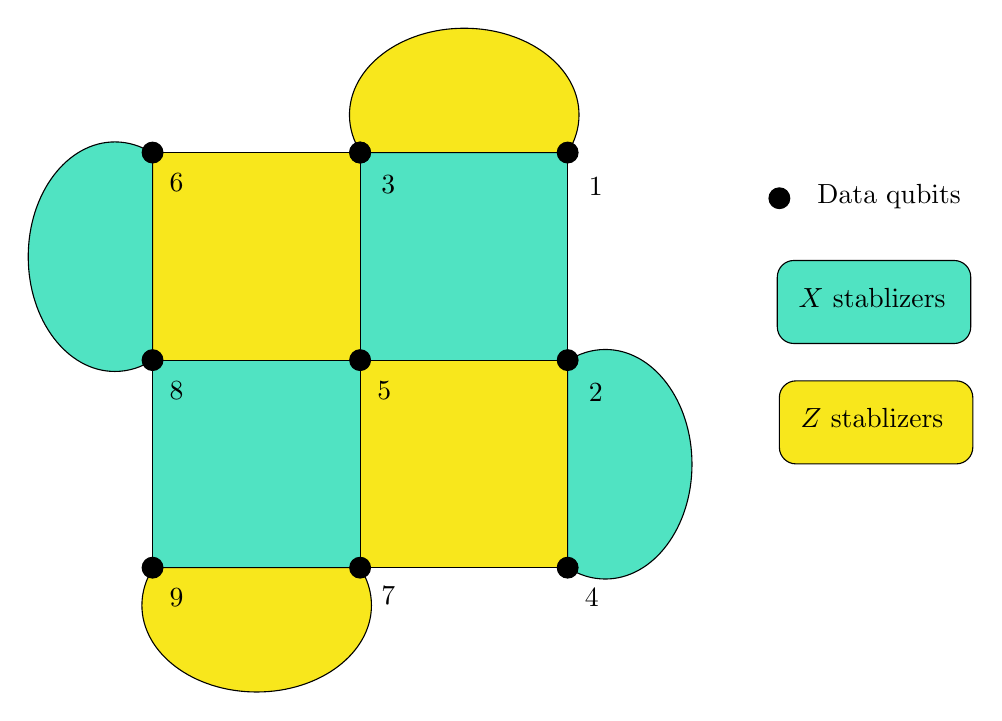
\begin{tikzpicture}[x=0.75pt,y=0.75pt,yscale=-1,xscale=1]
%uncomment if require: \path (0,380); %set diagram left start at 0, and has height of 380

%Shape: Grid [id:dp12900400367495535] 
\draw  [draw opacity=0][fill={rgb, 255:red, 80; green, 227; blue, 194 }  ,fill opacity=1 ] (109,74) -- (309,74) -- (309,274) -- (109,274) -- cycle ; \draw   (209,74) -- (209,274) ; \draw   (109,174) -- (309,174) ; \draw   (109,74) -- (309,74) -- (309,274) -- (109,274) -- cycle ;
%Shape: Grid [id:dp12880753916529475] 
\draw  [draw opacity=0][fill={rgb, 255:red, 248; green, 231; blue, 28 }  ,fill opacity=1 ] (109,74) -- (209,74) -- (209,174) -- (109,174) -- cycle ; \draw    ; \draw    ; \draw   (109,74) -- (209,74) -- (209,174) -- (109,174) -- cycle ;
%Shape: Grid [id:dp14038359941020084] 
\draw  [draw opacity=0][fill={rgb, 255:red, 248; green, 231; blue, 28 }  ,fill opacity=1 ] (209,174) -- (309,174) -- (309,274) -- (209,274) -- cycle ; \draw    ; \draw    ; \draw   (209,174) -- (309,174) -- (309,274) -- (209,274) -- cycle ;
%Shape: Chord [id:dp3348255380873256] 
\draw  [fill={rgb, 255:red, 80; green, 227; blue, 194 }  ,fill opacity=1 ] (109,174) .. controls (103.51,177.51) and (97.36,179.47) .. (90.86,179.47) .. controls (67.8,179.47) and (49.1,154.71) .. (49.1,124.17) .. controls (49.1,93.63) and (67.8,68.87) .. (90.86,68.87) .. controls (97.36,68.87) and (103.51,70.83) .. (109,74.34) -- cycle ;
%Shape: Chord [id:dp25355895312354426] 
\draw  [fill={rgb, 255:red, 248; green, 231; blue, 28 }  ,fill opacity=1 ] (209.34,74) .. controls (205.83,68.51) and (203.87,62.36) .. (203.87,55.86) .. controls (203.87,32.8) and (228.63,14.1) .. (259.17,14.1) .. controls (289.71,14.1) and (314.47,32.8) .. (314.47,55.86) .. controls (314.47,62.36) and (312.51,68.51) .. (309,74) -- cycle ;
%Shape: Chord [id:dp3710854401646404] 
\draw  [fill={rgb, 255:red, 80; green, 227; blue, 194 }  ,fill opacity=1 ] (309,174.34) .. controls (314.49,170.83) and (320.64,168.87) .. (327.14,168.87) .. controls (350.2,168.87) and (368.9,193.63) .. (368.9,224.17) .. controls (368.9,254.71) and (350.2,279.47) .. (327.14,279.47) .. controls (320.64,279.47) and (314.49,277.51) .. (309,274) -- cycle ;
%Shape: Chord [id:dp9474520489431058] 
\draw  [fill={rgb, 255:red, 248; green, 231; blue, 28 }  ,fill opacity=1 ] (209,274) .. controls (212.51,279.49) and (214.47,285.64) .. (214.47,292.14) .. controls (214.47,315.2) and (189.71,333.9) .. (159.17,333.9) .. controls (128.63,333.9) and (103.87,315.2) .. (103.87,292.14) .. controls (103.87,285.64) and (105.83,279.49) .. (109.34,274) -- cycle ;
%Shape: Circle [id:dp9459729009041369] 
\draw  [fill={rgb, 255:red, 0; green, 0; blue, 0 }  ,fill opacity=1 ] (104,74) .. controls (104,71.24) and (106.24,69) .. (109,69) .. controls (111.76,69) and (114,71.24) .. (114,74) .. controls (114,76.76) and (111.76,79) .. (109,79) .. controls (106.24,79) and (104,76.76) .. (104,74) -- cycle ;
%Shape: Circle [id:dp15256985423162583] 
\draw  [fill={rgb, 255:red, 0; green, 0; blue, 0 }  ,fill opacity=1 ] (304,74) .. controls (304,71.24) and (306.24,69) .. (309,69) .. controls (311.76,69) and (314,71.24) .. (314,74) .. controls (314,76.76) and (311.76,79) .. (309,79) .. controls (306.24,79) and (304,76.76) .. (304,74) -- cycle ;
%Shape: Circle [id:dp11883828343520664] 
\draw  [fill={rgb, 255:red, 0; green, 0; blue, 0 }  ,fill opacity=1 ] (204,74) .. controls (204,71.24) and (206.24,69) .. (209,69) .. controls (211.76,69) and (214,71.24) .. (214,74) .. controls (214,76.76) and (211.76,79) .. (209,79) .. controls (206.24,79) and (204,76.76) .. (204,74) -- cycle ;
%Shape: Circle [id:dp4998777753835695] 
\draw  [fill={rgb, 255:red, 0; green, 0; blue, 0 }  ,fill opacity=1 ] (204,74) .. controls (204,71.24) and (206.24,69) .. (209,69) .. controls (211.76,69) and (214,71.24) .. (214,74) .. controls (214,76.76) and (211.76,79) .. (209,79) .. controls (206.24,79) and (204,76.76) .. (204,74) -- cycle ;
%Shape: Circle [id:dp27945134021779117] 
\draw  [fill={rgb, 255:red, 0; green, 0; blue, 0 }  ,fill opacity=1 ] (104,174) .. controls (104,171.24) and (106.24,169) .. (109,169) .. controls (111.76,169) and (114,171.24) .. (114,174) .. controls (114,176.76) and (111.76,179) .. (109,179) .. controls (106.24,179) and (104,176.76) .. (104,174) -- cycle ;
%Shape: Circle [id:dp6684594543633622] 
\draw  [fill={rgb, 255:red, 0; green, 0; blue, 0 }  ,fill opacity=1 ] (304,174) .. controls (304,171.24) and (306.24,169) .. (309,169) .. controls (311.76,169) and (314,171.24) .. (314,174) .. controls (314,176.76) and (311.76,179) .. (309,179) .. controls (306.24,179) and (304,176.76) .. (304,174) -- cycle ;
%Shape: Circle [id:dp6456836036063145] 
\draw  [fill={rgb, 255:red, 0; green, 0; blue, 0 }  ,fill opacity=1 ] (204,174) .. controls (204,171.24) and (206.24,169) .. (209,169) .. controls (211.76,169) and (214,171.24) .. (214,174) .. controls (214,176.76) and (211.76,179) .. (209,179) .. controls (206.24,179) and (204,176.76) .. (204,174) -- cycle ;

%Shape: Circle [id:dp807085338591644] 
\draw  [fill={rgb, 255:red, 0; green, 0; blue, 0 }  ,fill opacity=1 ] (104,274) .. controls (104,271.24) and (106.24,269) .. (109,269) .. controls (111.76,269) and (114,271.24) .. (114,274) .. controls (114,276.76) and (111.76,279) .. (109,279) .. controls (106.24,279) and (104,276.76) .. (104,274) -- cycle ;
%Shape: Circle [id:dp905200708558098] 
\draw  [fill={rgb, 255:red, 0; green, 0; blue, 0 }  ,fill opacity=1 ] (304,274) .. controls (304,271.24) and (306.24,269) .. (309,269) .. controls (311.76,269) and (314,271.24) .. (314,274) .. controls (314,276.76) and (311.76,279) .. (309,279) .. controls (306.24,279) and (304,276.76) .. (304,274) -- cycle ;
%Shape: Circle [id:dp6226297152185722] 
\draw  [fill={rgb, 255:red, 0; green, 0; blue, 0 }  ,fill opacity=1 ] (204,274) .. controls (204,271.24) and (206.24,269) .. (209,269) .. controls (211.76,269) and (214,271.24) .. (214,274) .. controls (214,276.76) and (211.76,279) .. (209,279) .. controls (206.24,279) and (204,276.76) .. (204,274) -- cycle ;

%Rounded Rect [id:dp6080212331379622] 
\draw  [fill={rgb, 255:red, 80; green, 227; blue, 194 }  ,fill opacity=1 ] (410,134) .. controls (410,129.58) and (413.58,126) .. (418,126) -- (495.2,126) .. controls (499.62,126) and (503.2,129.58) .. (503.2,134) -- (503.2,158) .. controls (503.2,162.42) and (499.62,166) .. (495.2,166) -- (418,166) .. controls (413.58,166) and (410,162.42) .. (410,158) -- cycle ;
%Shape: Circle [id:dp09272358747691578] 
\draw  [fill={rgb, 255:red, 0; green, 0; blue, 0 }  ,fill opacity=1 ] (406,96) .. controls (406,93.24) and (408.24,91) .. (411,91) .. controls (413.76,91) and (416,93.24) .. (416,96) .. controls (416,98.76) and (413.76,101) .. (411,101) .. controls (408.24,101) and (406,98.76) .. (406,96) -- cycle ;
%Rounded Rect [id:dp47680208301511373] 
\draw  [fill={rgb, 255:red, 248; green, 231; blue, 28 }  ,fill opacity=1 ] (411,192) .. controls (411,187.58) and (414.58,184) .. (419,184) -- (496.2,184) .. controls (500.62,184) and (504.2,187.58) .. (504.2,192) -- (504.2,216) .. controls (504.2,220.42) and (500.62,224) .. (496.2,224) -- (419,224) .. controls (414.58,224) and (411,220.42) .. (411,216) -- cycle ;

% Text Node
\draw (428,88) node [anchor=north west][inner sep=0.75pt]   [align=left] {Data qubits};
% Text Node
\draw (419,138) node [anchor=north west][inner sep=0.75pt]   [align=left] {$\displaystyle X$ stablizers};
% Text Node
\draw (318,85) node [anchor=north west][inner sep=0.75pt]  [font=\normalsize] [align=left] {{\fontfamily{helvet}\selectfont 1}};
% Text Node
\draw (318,184) node [anchor=north west][inner sep=0.75pt]  [font=\normalsize] [align=left] {{\fontfamily{helvet}\selectfont 2}};
% Text Node
\draw (218,84) node [anchor=north west][inner sep=0.75pt]  [font=\normalsize] [align=left] {{\fontfamily{helvet}\selectfont 3}};
% Text Node
\draw (316,283) node [anchor=north west][inner sep=0.75pt]  [font=\normalsize] [align=left] {{\fontfamily{helvet}\selectfont 4}};
% Text Node
\draw (216,183) node [anchor=north west][inner sep=0.75pt]  [font=\normalsize] [align=left] {{\fontfamily{helvet}\selectfont 5}};
% Text Node
\draw (116,83) node [anchor=north west][inner sep=0.75pt]  [font=\normalsize] [align=left] {{\fontfamily{helvet}\selectfont 6}};
% Text Node
\draw (218,282) node [anchor=north west][inner sep=0.75pt]  [font=\normalsize] [align=left] {{\fontfamily{helvet}\selectfont 7}};
% Text Node
\draw (116,183) node [anchor=north west][inner sep=0.75pt]  [font=\normalsize] [align=left] {{\fontfamily{helvet}\selectfont 8}};
% Text Node
\draw (116,283) node [anchor=north west][inner sep=0.75pt]  [font=\normalsize] [align=left] {{\fontfamily{helvet}\selectfont 9}};
% Text Node
\draw (420,196) node [anchor=north west][inner sep=0.75pt]   [align=left] {$\displaystyle Z$ stablizers};


\end{tikzpicture}
\end{document}